% This LaTeX document needs to be compiled with XeLaTeX.
\documentclass[
  10
]{article}
\usepackage[margin=2cm,includehead=true,includefoot=true,centering,]{geometry}
\usepackage{xcolor}
\usepackage{ucharclasses}
\usepackage{hyperref}
\usepackage{amsmath,amssymb}
\usepackage{amsfonts}
\usepackage[version=4]{mhchem}
\usepackage{stmaryrd}
\usepackage{bbold}
\usepackage{polyglossia}
\usepackage{fontspec}
\usepackage{ctex}
\usepackage[export]{adjustbox}
\usepackage{tabularx}
\usepackage{booktabs}

\usepackage{setspace}
\setstretch{1.2}

\makeatletter
\@ifundefined{KOMAClassName}{% if non-KOMA class
  \IfFileExists{parskip.sty}{%
    \usepackage{parskip}
  }{% else
    \setlength{\parindent}{0pt}
    \setlength{\parskip}{6pt plus 2pt minus 1pt}}
}{% if KOMA class
  \KOMAoptions{parskip=half}}
\makeatother
\usepackage{longtable,booktabs,array}
\newcounter{none} % for unnumbered tables
\usepackage{calc} % for calculating minipage widths
% Correct order of tables after \paragraph or \subparagraph
\usepackage{etoolbox}
\makeatletter
\patchcmd\longtable{\par}{\if@noskipsec\mbox{}\fi\par}{}{}
\makeatother
% Allow footnotes in longtable head/foot
\IfFileExists{footnotehyper.sty}{\usepackage{footnotehyper}}{\usepackage{footnote}}
\makesavenoteenv{longtable}
\usepackage{graphicx}
\makeatletter
\newsavebox\pandoc@box
\newcommand*\pandocbounded[1]{% scales image to fit in text height/width
  \sbox\pandoc@box{#1}%
  \Gscale@div\@tempa{\textheight}{\dimexpr\ht\pandoc@box+\dp\pandoc@box\relax}%
  \Gscale@div\@tempb{\linewidth}{\wd\pandoc@box}%
  \ifdim\@tempb\p@<\@tempa\p@\let\@tempa\@tempb\fi% select the smaller of both
  \ifdim\@tempa\p@<\p@\scalebox{\@tempa}{\usebox\pandoc@box}%
  \else\usebox{\pandoc@box}%
  \fi%
}
% Set default figure placement to htbp
\def\fps@figure{htbp}
\makeatother
\setlength{\emergencystretch}{3em} % prevent overfull lines
\providecommand{\tightlist}{%
  \setlength{\itemsep}{0pt}\setlength{\parskip}{0pt}}


\hypersetup{colorlinks=true, linkcolor=blue, filecolor=magenta, urlcolor=cyan,}
\urlstyle{same}

\usepackage{colortbl}
\definecolor{table-row-color}{HTML}{999999}
\definecolor{table-rule-color}{HTML}{999999}
%\arrayrulecolor{black!40}
\arrayrulecolor{table-rule-color}     % color of \toprule, \midrule, \bottomrule
\setlength{\aboverulesep}{0pt}
\setlength{\belowrulesep}{0pt}


\setotherlanguages{english}
\IfFontExistsTF{Source Han Serif CN}
{\newfontfamily\chinesefont{Source Han Serif CN}}
{\IfFontExistsTF{Noto Serif CJK SC}
  {\newfontfamily\chinesefont{Noto Serif CJK SC}}
  {\IfFontExistsTF{SimSun}
    {\newfontfamily\chinesefont{SimSun}}
    {\IfFontExistsTF{FangSong}
      {\newfontfamily\chinesefont{FangSong}}
      {\newfontfamily\chinesefont{Arial Unicode MS}}
}}}
\IfFontExistsTF{Times New Roman}
{\newfontfamily\englishfont{Times New Roman}}
{\IfFontExistsTF{Liberation Serif}
  {\newfontfamily\englishfont{Liberation Serif}}
  {\IfFontExistsTF{DejaVu Serif}
    {\newfontfamily\englishfont{DejaVu Serif}}
    {\newfontfamily\englishfont{Arial}}
}}


\author{}
\date{}

\begin{document}


\section{第十五届（2022 年）}\label{ux7b2cux5341ux4e94ux5c4a2022-ux5e74}

\section{北京市大学生物理实验竞赛}\label{ux5317ux4eacux5e02ux5927ux5b66ux751fux7269ux7406ux5b9eux9a8cux7adeux8d5b}

\section{参赛项目说明书}\label{ux53c2ux8d5bux9879ux76eeux8bf4ux660eux4e66}

参赛题目 ：（请画选择）

题目一：用经典物理系统模拟一些量子物理现象或技术。

题目二：研究物质的折射特性，并利用该特性制作一个实际应用装置。

题目三：实验制作（□定量类 □演示类）

题目四：论文（□教学型 □科研型）

北京市大学生物理实验竞赛组委会制

2022 年 9 月

\subsection{基于锥形无芯光纤的湿度传感器的研制}\label{ux57faux4e8eux9525ux5f62ux65e0ux82afux5149ux7ea4ux7684ux6e7fux5ea6ux4f20ux611fux5668ux7684ux7814ux5236}

\subsection{和论文类填写）}\label{ux548cux8bbaux6587ux7c7bux586bux5199}

\subsection{设计原理：}\label{ux8bbeux8ba1ux539fux7406}

空气的折射率会随着空气湿度的改变而改变，根据空气的此折射特性，本小组设计了一种基于锥形无芯光纤的湿度传感器。传统的电感、电容湿度传感器具有很多优点，如响应速度快、易于测量等。然而，它们却受到电路漏电的影响，而且测量精度不够高。随着科技的不断进步发展，光学类湿度传感器由于其高集成度、高灵敏度、适用范围广等优点而被人们广泛关注，本实验设计的基于锥形无芯光纤的湿度传感器灵敏度高、易于控制且适用范围广，便于实际应用。

\subsection{一、空气的折射特性}\label{ux4e00ux7a7aux6c14ux7684ux6298ux5c04ux7279ux6027}

1965年Edlen提出的湿度对折射率的影响公式为：

\[
n _ {t p f} - n _ {t p} = - f [ 3. 7 3 4 5 - 0. 0 4 0 1 * \sigma^ {2} ] \times 1 0 ^ {- 1 0}\tag{1}
\]

式(1)中， \(n _ { t p f }\) 和 \(n _ { t p }\)
为分别为相同的潮湿空气和干燥空气的折射率，
\(\sigma _ { \mathcal { A } } ^ { \cdot }\) 为真空中光的波数，单位为
\(1 \mu \mathrm { m } ^ { - 1 }\) 。水蒸气分压力�与饱和蒸汽压
\({ \mathrm { j } } _ { 0 }\) 的关系为：

\[
f = f _ {0} * \mathrm{R}\tag{2}
\]

（2）式中，R 为相对湿度。由此可知，在其他参数不变的条件下，水蒸气分压力
\(f ^ { \bot }\) 相对湿度成正比。空气湿度增大时，水蒸气分压力�增大，
\(n _ { t p f } - n _ { t p }\) 减小，由 \(\mp n _ { t p }\)
不变，导致空气折射率 \({ \cdot } n _ { t p f }\)
减小，反之空气湿度减小时，空气折射率 \(\cdot n _ { t p f }\) 增大。

取波长 \(\lambda { = } 1 5 5 0 \ \mathrm { n m } ,\) ，大气压强
P=1013hPa，温度
\(\mathrm { t } { = } 2 0 \mathrm { { } ^ { \circ } C }\)
，湿度取值区间为(0, 100\%)，考察湿度对空气折射率值的影响，计算结果如图
1所示。

\pandocbounded{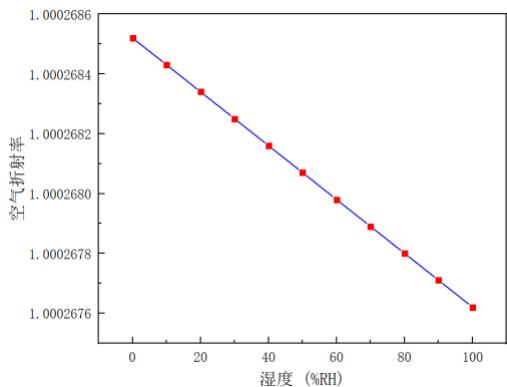
\includegraphics[keepaspectratio,alt={image}]{images/171ab5c4ba9c2f23b9ea4731fee3bdbf2df4703f660e5cc0d04c78a17a9c354e.jpg}}

图 1 湿度对折射率的影响（计算值）

从计算结果可以看出，在保持光波长和大气压温度等参数不变时，空气湿度值与空气折射率值成线性关系，根据空气的此折射特性本小组设计了基于锥形无芯光纤的湿度传感器。

\subsection{二、基于空气折射特性的湿度传感器的基本原理}\label{ux4e8cux57faux4e8eux7a7aux6c14ux6298ux5c04ux7279ux6027ux7684ux6e7fux5ea6ux4f20ux611fux5668ux7684ux57faux672cux539fux7406}

\subsection{（1）基于光纤倏逝波的传感原理}\label{ux57faux4e8eux5149ux7ea4ux500fux901dux6ce2ux7684ux4f20ux611fux539fux7406}

全光纤传感探头采用单模-无芯-单模结构，简称 SNS如图 2所示。

\pandocbounded{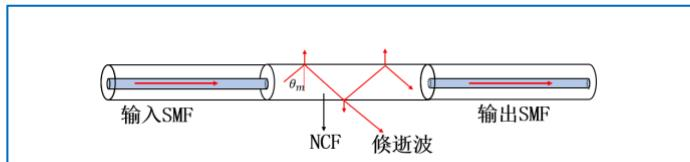
\includegraphics[keepaspectratio,alt={image}]{images/2a91d1485bf5fa8e8399b897699f16466498bda0a6967e674d022d8a34797140.jpg}}

图 2 SNS 全光纤传感探头的结构

外界空气充当无芯光纤 NCF的包层，由于NCF的直径远大于单模光纤
SMF的纤芯直径，因此当输入光传输至NCF时，会在
NCF中激发起多个模式。各阶模式在
NCF与外界空气的界面上发生折射，会在透入一定深度的外界空气中形成倏逝场，外界空气会对倏逝场有一定的衰减作用，所以当光波通过长度为�的NCF后，可推导出光在波长�处的透射率公式：

\[
T (\lambda) = \sum_ {m \cdot n = 1} ^ {M} c _ {m} ^ {2} \cdot c _ {n} ^ {2} \cdot \cos [ (\beta_ {m} - \beta_ {n}) L ] \cdot \exp [ - (\gamma_ {m} + \gamma_ {n}) L ]\tag{3}
\]

(3)式中激发系数 \(. c _ { m }\) 、模式干涉项
\(\mathrm { \backslash } c o s [ ( \beta _ { m } - \beta _ { n } ) L ]\)
和衰减项 \(e x p [ - ( \gamma _ { m } + \gamma _ { n } ) L ]\)
均随着空气湿度的变化而变化，这样透射光谱也会随着空气湿度的变化而改变，具体反映在干涉项变化引起的特征峰的移动和三项共同作用引起的透射率变化。影响透射谱透射率的激发系数
\(. c _ { m }\) 、模式传播常数 \(\cdot \beta _ { m }\) 和倏逝场衰减系数
\(\cdot \gamma _ { m }\)
均与波长�有关，因此在其他参数相同的条件下，相同的空气湿度下不同波长处的传输损耗不同；同样在空气湿度相同的条件下，不同波长处透射损耗的变化也不同。因此，可以通过透射谱特征波长的移动和传感探头透射功率的变化来检测空气的湿度。

\subsection{（2）锥形NCF传感增敏原理}\label{ux9525ux5f62ncfux4f20ux611fux589eux654fux539fux7406}

为了提高灵敏度，采用单模-锥形NCF单模结构作为传感探头，锥形光纤示意图如图
3所示。某一特定波长的光从锥形光纤的大端面向小端面入射时，入射角
\(\alpha _ { n }\)
随次数�增加而不断减小，如图3（a）所示，由倏逝波的定义可知穿透深度如（4）式所示。

\[
d _ {t} = \frac {\lambda}{2 \pi \sqrt {n _ {1} ^ {2} s i n ^ {2} \theta_ {i} - n _ {2} ^ {2}}}\tag{4}
\]

由此可知，在波长一定情况下，随反射次数的增加 \(\lvert d _ { t }\)
不断增大。在接近临界角的情况下， \(d _ { t }\)
急剧增大。某一特定波长的光从锥形光纤的小端面向大端面入射时，如图3（b）所示，由公式（4）可知，随着反射次数的增加之
\(d _ { t }\) 不断减小。在接近 \(9 0 ^ { \circ }\) 的情况下，
\(d _ { t }\) 趋于平稳，对光的束缚能力也达到最大。 \(d _ { t }\)
决定了光场能量泄露与外界物质的相互作用的大小。因此，采用锥形光纤增加
\(\scriptstyle 1 d _ { t }\) ，可以提高湿度传感器的灵敏度。

\pandocbounded{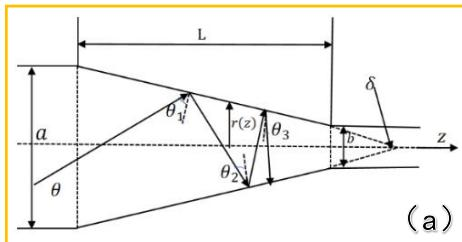
\includegraphics[keepaspectratio,alt={image}]{images/76d421b90583209a292743ba12a55ebb8515e6564e57040a9644c98123475f68.jpg}}

\pandocbounded{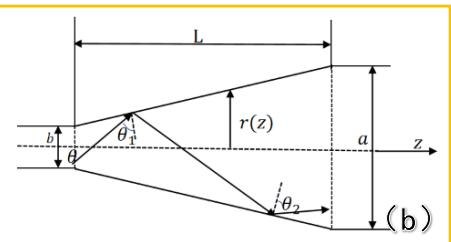
\includegraphics[keepaspectratio,alt={image}]{images/9a75864af6048fc1dd4f6cd6873f6ce4f02a62a26b8dbe0eb4c8746fea8dbdac.jpg}}

图 3 锥形光纤示意图
（a）光波从大端面向小端面入射（b）光波从小端面向大端面入射

\subsection{（3）传感系统设计原理}\label{ux4f20ux611fux7cfbux7edfux8bbeux8ba1ux539fux7406}

为了直观显示所测外界空气的湿度值，设计了光纤传感系统。系统包括：光纤传感模块（光源和
SNS
传感探头）、单片机控制模块、实现各种功能的硬件电路（光电检测模块、信号放大与
A/D转换电路）以及显示模块，整个系统设计的原理框图如图4
所示。光纤传感模块产生的光信号传递到光电检测模块，将光信号转换成电信号后传送到下一级的放大与
转换电路，处理后的信号通过通信接口连接到控制模块，由控制模块计算并最后在显示模块上实时显示出外界空气的湿度值。

\pandocbounded{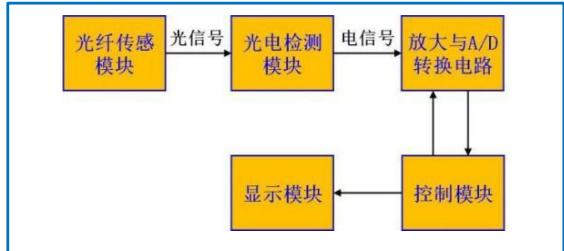
\includegraphics[keepaspectratio,alt={image}]{images/fff28fa08e65fb837c5e53276ada4c86ba7f72f6676f4dff9e65509812c95634.jpg}}

图 4 传感系统示意图

\subsection{设计方法：}\label{ux8bbeux8ba1ux65b9ux6cd5}

\subsection{（1）制作SNS结构的光纤传感探头}\label{ux5236ux4f5csnsux7ed3ux6784ux7684ux5149ux7ea4ux4f20ux611fux63a2ux5934}

首先，取一根2米长的单模光纤跳线，用剪刀截成两段，再用剥线钳剥离光纤护套，控制剥线长度在40mm左右，使用无纺布蘸取少量酒精，顺光纤轴向擦去光纤表面残留的碎屑，再使用光纤切割刀将光纤端面切平整。无芯光纤的端面处理与上面步骤相同。将处理好端面的无芯光纤与单模光纤放入熔接机的V型槽，合上压板，关闭防风盖，进行熔接。同理，继续熔接无芯光纤与另外一根单模光纤，形成SNS光纤结构的传感探头。

\subsection{（2）制作锥形NCF传感探头}\label{ux5236ux4f5cux9525ux5f62ncfux4f20ux611fux63a2ux5934}

为增加传感探头的灵敏度，本实验在SNS结构的基础上对NCF进行拉锥处理。用熔融拉锥机制作锥形NCF。对拉锥机参数进行设置，待拉伸长度达到3500μm时，形成锥形NCF传感探头。

为了对比 NCF、锥形 NCF 形貌上的差别，我们使用 SEM
对上述两种光纤进行观测，其结果如图5
所示，从图(a)和图(b)中可以看到，NCF的直径约为
125μm，拉锥处理后光纤直径明显变细，约为20μm。

\pandocbounded{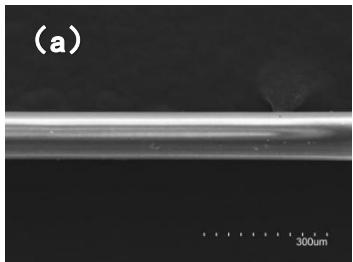
\includegraphics[keepaspectratio,alt={image}]{images/a4a5e2ced2e983f2d0f96c2673c4014419243b09b0d5ec13b8a1c168820cdabc.jpg}}

图 5 两种光纤的SEM 照片

\pandocbounded{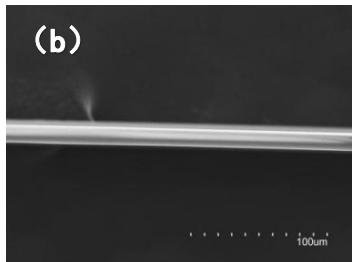
\includegraphics[keepaspectratio,alt={image}]{images/e4feb13721e88aa3fd564e493b4c47fde829d1212e5f331bbff041fc13eb2467.jpg}}

（a）NCF （b）锥形 NCF

\subsection{实验仪器与装置:}\label{ux5b9eux9a8cux4eeaux5668ux4e0eux88c5ux7f6e}

单模光纤(SMF-28)，无芯光纤
(CL1010-A)，剥线钳，切割刀，酒精，无纺布，熔接机（INNO
IFS-15M），宽带光源（NKT DK-3460），光谱仪（Yokogawa AQ6370C），1550nm
激光器（KF-184A），功率计（JW3208），3dB
耦合器，熔融拉锥机（AFBT-6000），湿度计，加湿器,STM32F103
系列开发板，1GHz光电探测器，掺铒光纤放大器（Thorlabs EDFA100S），ADS115
电路模块

\subsection{数据测量与分析：}\label{ux6570ux636eux6d4bux91cfux4e0eux5206ux6790}

将SNS结构的传感探头置入用亚克力板切割粘合而成的湿度控制箱中，通过跳线一端连接宽带光源，另一端连接光谱仪。光从宽带光源(波长范围
1525-1610nm)耦合进传感探头。透射光谱由分辨率为 0.02nm 的光谱仪(Yokogawa
AQ6370C)记录。通过光谱仪测量不同湿度下 NCF
透射谱变化规律，如图6所示，（a）为原理示意图，（b）为实物装置图，（c）为
SNS传感探头在不同湿度下的透射光谱。

\pandocbounded{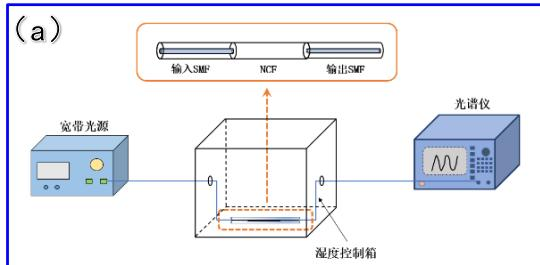
\includegraphics[keepaspectratio,alt={image}]{images/b89627bec7752a1552fdd370b9bc665443978458f009a3c505d6cd9c9ef89e84.jpg}}

\pandocbounded{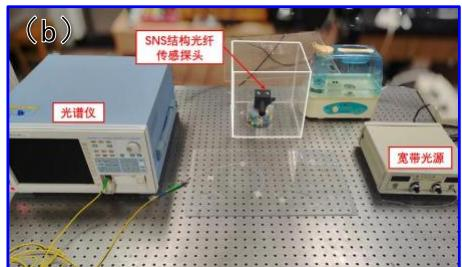
\includegraphics[keepaspectratio,alt={image}]{images/fd000fb28697ad716710240e447e400f3e907c615771cf5c32c86330a2bda4f6.jpg}}

\pandocbounded{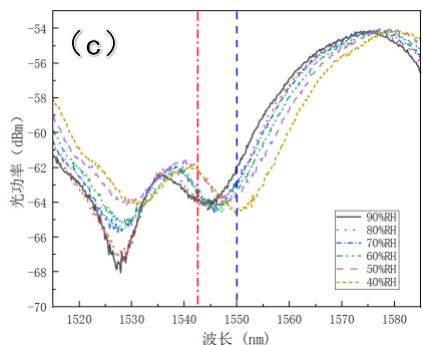
\includegraphics[keepaspectratio,alt={image}]{images/bb72425eeb943ad4cac7137011667628f54f546e9eaa6ac92453367da091d060.jpg}}

图 6 SNS 结构的传感特性测试 （a）测量透射光谱装置示意图
（b）测量透射光谱装置实物图(c)不同湿度下的透射光谱

由图6（c）可知，在
1550nm处（图中竖条蓝线位置），传感器输出端的光功率随湿度的增大不断增大。如果波长选在1542.5nm处（图中竖条红线位置），则输出光功率随湿度的增大不断减小。

为了直观显示空气的湿度值，将光源波长固定在
1550nm处，测量功率变化与湿度的关系。分别将两种结构的传感探头置入湿度控制箱中，光从1550nm
激光器发出，进入3dB耦合器，耦合器一端连接功率计
1，用来监测光源的功率变化，若变化太大，就调节光源电流让其稳定在初始值；另一端连接传感探头，外界空气的湿度发生变化时，传感探头输出的光功率也会发生变化，功率计2用来测量经过传感探头后功率的变化。如图7所示，（a）为实验装置示意图，（b）为实验装置实物图。

\pandocbounded{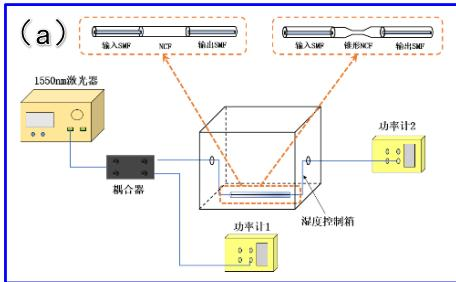
\includegraphics[keepaspectratio,alt={image}]{images/8d314eea148f84bea7c31dba86dbb80a1ca2a5d84a881f9090b5f9bdb2e7568d.jpg}}

\pandocbounded{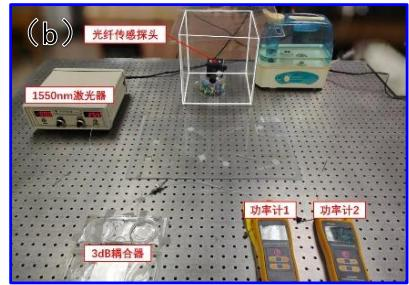
\includegraphics[keepaspectratio,alt={image}]{images/8dba65bcb577aa4b65556c65d6afacda3518c99bdcd6ab57556fc45ed67f3210.jpg}}

图 7 （a）实验装置示意图 （b）实验装置实物图

依次记录连接 SNS 光纤传感探头和锥形 NCF
传感探头在空气中功率随外界空气湿度变化的数据，使用Origin软件对所得实验数据拟合，绘制出各结构的光纤传感探头功率随湿度变化曲线如图8
所示。

\pandocbounded{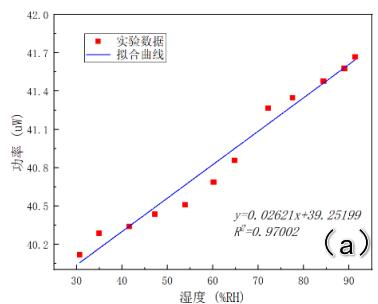
\includegraphics[keepaspectratio,alt={image}]{images/f0ad66d177e7da84e46447fa5305a1206262d20e99fc243a46733c78027bc8f4.jpg}}

\pandocbounded{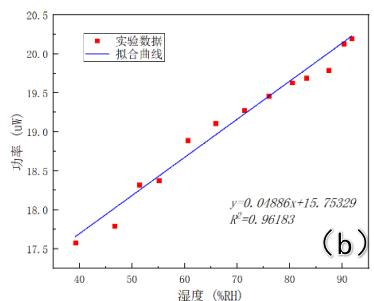
\includegraphics[keepaspectratio,alt={image}]{images/326c6e21172c7e3f40a432b9ad720df2cc63aecc91829529ea5064e4f8e2f0da.jpg}}

图8 传感探头功率随湿度的变化（a）NCF（b）锥形 NCF

由图8（a）可知，SNS
光纤传感探头功率随湿度变化呈现出良好的线性关系。其拟合的线性关系为
\(\mathrm { y } { = } 0 . \ 0 2 6 2 \mathrm { x } { + } 3 9 . \ 2 5 2 0\)
，灵敏度为 26.21nW/\%RH，相关系数为 0.9700。由图 8（b）可知，锥形
NCF传感探头功率随湿度变化的拟合线性关系为
\(\mathrm { y } { = } 0 . \ 0 4 8 9 \mathrm { x } { + } 1 5 . \ 7 5 3 3\)
，其灵敏度为 48.86nW/\%RH，相关系数为 0.9618。由此可知，采用锥形
NCF探头传感，灵敏度提高了。通过对所测的数据进行分析：平均误差为±1.98\%RH，最大误差为
4.81\%RH，最小误差为 0.08\%RH。可以看到，锥形
NCF传感探头的测量误差很小，可以满足实际应用的需求。

为了直观显示所测的湿度值，采用锥形NCF的传感探头，加入数据处理显示系统。从传感探头输出的光信号，经过光放大器后放大，进入光电探测器转化为电信号，传送到下一级的A/D转换电路，处理后的信号通过通信接口连接到单片机，由单片机计算并最后在显示模块上实时显示出空气湿度值。如图9所示，（a）为原理示意图，（b）为实物装置图。

\pandocbounded{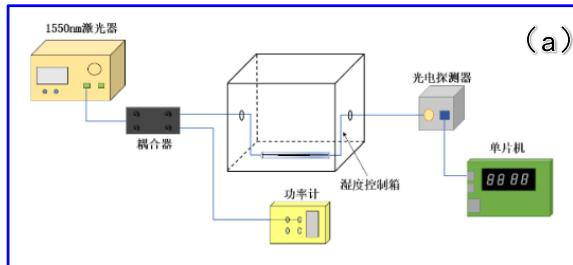
\includegraphics[keepaspectratio,alt={image}]{images/9e7cc2c709acc99556ea86e288c94e8e0424ea1ec2a93e55506ba96f184d9772.jpg}}

\pandocbounded{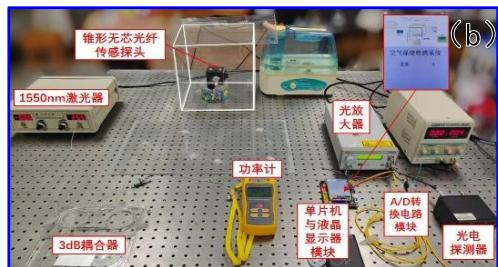
\includegraphics[keepaspectratio,alt={image}]{images/10b5e22bda78f18fe4daba9b4fb3aece1fca1a1a225d512cb53a14e3dcb6d363.jpg}}

图 9 基于锥形 NCF 传感探头的湿度测量系统
（a）实验装置示意图（b）实验装置实物图

实时测量空气湿度，实际湿度值和单片机所显示的测量湿度值及两者间的误差如表
1所示。

\subsection{表 1
湿度实际值、测量值和误差}\label{ux8868-1-ux6e7fux5ea6ux5b9eux9645ux503cux6d4bux91cfux503cux548cux8befux5dee}

{\def\LTcaptype{none} % do not increment counter
\begin{longtable}[]{@{}|l|l|l|@{}}
\toprule\noalign{}
\endhead
\bottomrule\noalign{}
\endlastfoot
\hline
实际湿度值 & 测量湿度值 & 误差 \\
\hline
38.9\% & 37.951\% & 0.949\% \\
\hline
46.2\% & 46.857\% & -0.657\% \\
\hline
50.7\% & 52.162\% & -1.462\% \\
\hline
54.5\% & 53.983\% & 0.517\% \\
\hline
60.3\% & 61.475\% & -1.175\% \\
\hline
66.9\% & 66.086\% & 0.814\% \\
\hline
72.4\% & 73.839\% & -1.439\% \\
\hline
76.8\% & 75.850\% & 0.950\% \\
\hline
81.1\% & 81.994\% & -0.894\% \\
\hline
85.3\% & 84.712\% & 0.588\% \\
\hline
89.0\% & 87.638\% & 1.362\% \\
\hline
90.3\% & 89.121\% & 1.179\% \\
\hline
93.2\% & 94.442\% & -1.242\% \\
\hline
\end{longtable}
}

当在 40～95\%RH 的湿度范围内：平均误差为±1.02\%RH，最大误差为
1.462\%RH，最小误差为0.588\%RH。此种基于锥形无芯光纤的湿度传感器与一定范围的实际湿度的平均误差范围很小，具有很好的准确性和实时性。

\subsection{结论：}\label{ux7ed3ux8bba}

本实验基于锥形无芯光纤的传感特性研制了一种测量空气湿度的传感系统，可直接将光纤传感探头置入湿度控制箱，通过单片机以及液晶显示模块实时显示湿度值，对空气湿度的测量范围可以从
40 到 95\%RH，测量范围较为广泛。通过对 SNS
结构的无芯光纤拉锥处理，能显著提高测试灵敏度，对于湿度的灵敏度可以实现从
26.21nW/\%RH 增加到
48.86nW/\%RH。这种基于锥形无芯光纤的湿度传感器简单小巧且适用范围广，提高了湿度测量的灵敏度与稳定性。

\subsection{项目创新与特色：}\label{ux9879ux76eeux521bux65b0ux4e0eux7279ux8272}

\subsection{（1）SNS结构光纤传感探头的优势}\label{snsux7ed3ux6784ux5149ux7ea4ux4f20ux611fux63a2ux5934ux7684ux4f18ux52bf}

相较于传统的湿度传感器，光纤传感器价格低廉，体积小、重量轻且制备简单。

\subsection{（2）锥形NCF传感探头提高传感精度}\label{ux9525ux5f62ncfux4f20ux611fux63a2ux5934ux63d0ux9ad8ux4f20ux611fux7cbeux5ea6}

一般情况下，基于无芯光纤的SNS结构的灵敏度不够高（本实验中测量空气湿度灵敏度为：26.21nW/\%RH），而采用的基于锥形无芯光纤的
SNS 结构能够很好的提高传感器的灵敏度（腰锥直径为20μm，灵敏度为
48.86nW/\%RH）。

\subsection{（3）系统可以实现空气湿度实时显示}\label{ux7cfbux7edfux53efux4ee5ux5b9eux73b0ux7a7aux6c14ux6e7fux5ea6ux5b9eux65f6ux663eux793a}

本实验系统可以在外接屏幕上实时显示空气湿度的数值。系统简单、小巧，易于控制且适用范围广。为该基于锥形无芯光纤的湿度传感器的实际应用推广奠定了基础。

\subsection{制作成本（明细）：}\label{ux5236ux4f5cux6210ux672cux660eux7ec6}

{\def\LTcaptype{none} % do not increment counter
\begin{longtable}[]{@{}|l|l|l|l|@{}}
\toprule\noalign{}
\endhead
\bottomrule\noalign{}
\endlastfoot
\hline
名称 & 数量 & 单价(元) & 总价(元) \\
\hline
3 米单模光纤 & 3 & 30 & 90 \\
\hline
1 米无芯光纤 & 1 & 150 & 150 \\
\hline
3dB 耦合器 & 1 & 100 & 100 \\
\hline
模数转换模块 & 1 & 30 & 30 \\
\hline
STM32 单片机、显示屏 & 1 & 318 & 318 \\
\hline
总计 & \multicolumn{3}{l@{}}{%
688 元} \\
\hline
\end{longtable}
}

\end{document}
